\documentclass[10pt,a4paper]{article}
\usepackage[a4paper, top=2cm, bottom=1.5cm, left=1.5cm, right=1.5cm]{geometry} % Задать размеры полей.
\usepackage[warn]{mathtext} % Русские символы в формулах. Нужно писать до пакета babel. Указывает, что в формулах используются символы кириллицы, которые по умолчанию печатаются прямым шрифтом.
\usepackage[T2A]{fontenc}
\usepackage[utf8]{inputenc}
\usepackage[russian]{babel}
\usepackage{amsmath}
\usepackage{amssymb}
\usepackage{graphicx}
%\usepackage{floatrow}
\usepackage{booktabs}
\usepackage{wrapfig}
\usepackage{fancyhdr}
\usepackage{multicol}
\usepackage{xcolor}

\usepackage{float}
\usepackage{multirow}

% Объявляем новую команду для переноса строки внутри ячейки таблицы
\newcommand{\specialcell}[2][c]{%
	\begin{tabular}[#1]{@{}c@{}}#2\end{tabular}}

\newcommand{\figref}[1]{(См. рис. \ref{#1})}
\newcommand{\secref}[1]{(См. раздел. \ref{#1})}

\newcommand{\angstrom}{\text{\normalfont\AA}}
\newcommand{\e}[1]{\text{$\cdot10^{#1}$}}
\newcommand{\m}{\; м}
\newcommand{\mm}{\; мм}
\newcommand{\um}{\; мкм}
\newcommand{\A}{\; А}
\newcommand{\uV}{\; мкВ}
\newcommand{\cels}{\; ^\circ С}

\pagestyle{fancy}
\fancyhead{}
\fancyhead[L]{\small Дедков Д.А., Маслов А.С., Экспериментальная проверка уравнения Эйнштейна для фотоэффекта и определение постоянной Планка. МФТИ, 2023 г.}
\fancyhead[R]{}
\fancyfoot[C]{\thepage}

\renewcommand{\cot}{\text{ctg}}

\author{\normalsize Дедков Денис, Маслов Артём \\
	\normalsize группа Б01-108а \\
	\normalsize 02.10.2023}
\date{}

\title{
	\Large Экспериментальная проверка уравнения Эйнштейна для фотоэффекта и определение постоянной Планка \\ 
}

\begin{document}
\maketitle
	
	\subsection*{Цель и задачи работы:}
	\begin{enumerate}
		\item Исследовать зависимость величины фототока от задерживающего потенциала и частоты падающего излучения.
		
		\item Вычислить величину постоянной Планка.
	\end{enumerate}
	
	\subsection*{Описание экспериментальной установки}
	
	Схема экспериментальной установки приведена на рисунке \ref{img:exp_scheme}:
	\begin{figure}[H]
		\centering
		\begin{minipage}[c]{0.48\textwidth}
			\centering
			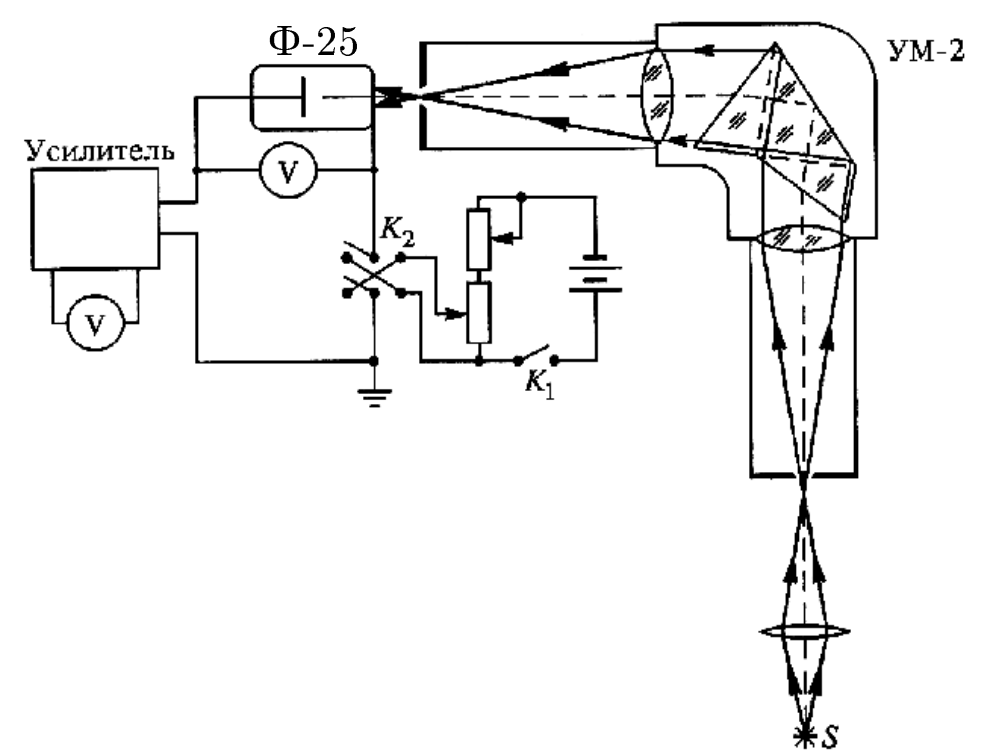
\includegraphics[width=0.8\textwidth]{images/exp_scheme.png}
			\caption{Схема экспериментальной установки.}
			\label{img:exp_scheme}
		\end{minipage}
		\hfill
		\begin{minipage}[c]{0.48\textwidth}
			\centering
			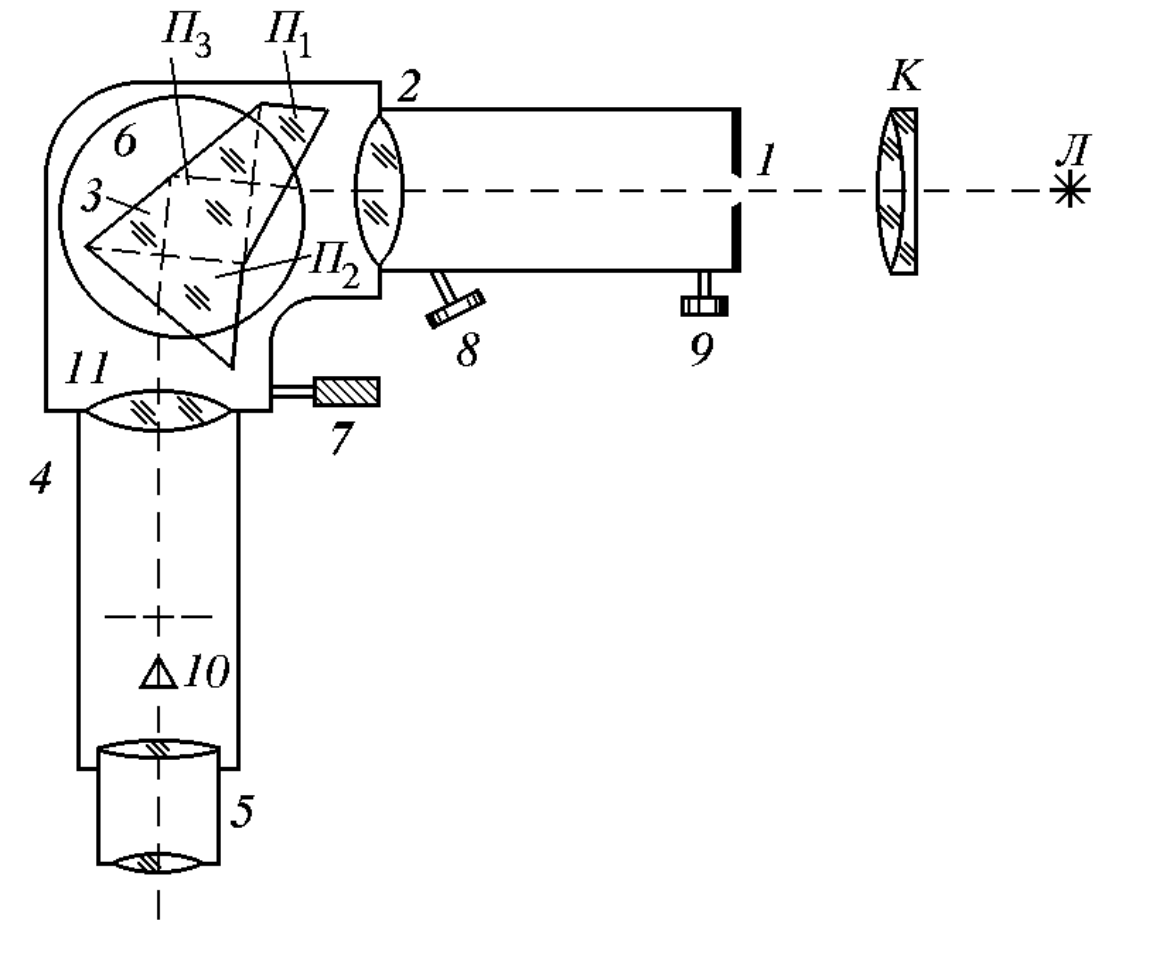
\includegraphics[width=0.8\textwidth]{images/exp_scheme2.png}
			\caption{Схема монохроматора.}
			\label{img:exp_scheme2}
		\end{minipage}
	\end{figure}

	Излучения источника $S$ фокусируется на входную щель призменного монохроматора УМ-2, выделяющего узкий спектральный интервал, и попадает на катод фотоэлемента Ф-25.
	
	Рассмотрим схему монохроматора рисунок \ref{img:exp_scheme2}. Входная щель 1 снабжена микрометрическим винтом 9 для регулировки нужной ширины щели. Коллиматорный объектив 2 имеет микрометрический винт 8, который позволяет смещать объектив относительно щели при фокусировке различных спектральных линий. Спектральная призма 3 выделяет узкую линию спектра падающего излучения. Поворотный столик 6 позволяет и барабан 7 с делениями позволяют наводиться на нужную спектральную линию. Зрительная труба, состоящая из объектива 4 и окуляра 5, позволяет проградуировать барабан на спектральные линии. При измерениях зрительная трубка заменяется блоком фотодетектора. 
	
	Фототок на фотоэлемента усиливается усилителем и напряжение, пропорциональное току измеряется вольтметром. Величина задерживающего напряжение фотоэлемента измеряется вторым вольтметром. Величину задерживающего напряжения можно регулировать с помощью блока питания.

	\subsection*{Оборудование и приборы}
	
	Экспериментальная установка $№1.1_4$.
	
	\begin{enumerate}
		\item Фотоэлемент Ф-25.
		
		\item Призменный монохроматор УМ-2. Рабочий диапазон от $0.38 \um$ до $1.00 \um$. Инвентарный номер №410134125745. Заводской номер №51026.
		
		\item Неоновая лампа.
		
		\item Лампа накаливания К-12.
		
		\item Вольтметры GDM-8145. Инвентарный номер вольтметра, измеряющего напряжение пропорциональное фототоку, №51391. Инвентарный номер вольтметра, измеряющего задерживающее напряжение, №51399. Погрешность измерения постоянного напряжения $\sigma = \pm (0.03\% rdg + 4 digits)$
		
		\item Блок питания. Инвентарный номер №410134125745.
	\end{enumerate}
	
	\subsection*{Первичные экспериментальные данные}
	
	В таблице 1 приведены данные градуировки монохроматора. $\lambda$ -- длина спектральной линии ${}^{10}Ne$, $N$ -- отсчёты в градусах, соответствующие данной спектральной линии.
	
	\begin{tabular}{ccc}
		\begin{tabular}[t]{c}
			Таблица 1.\\Градуировка\\призменного\\ монохроматора. \\
			\input{gen/tab-calib.tex}
		\end{tabular}&
		
		\begin{tabular}[t]{c}
			Таблица 2. Длина волны $7032.41 \angstrom$. \\
			\input{gen/tab-data-2992.tex}
		\end{tabular}&
	
		\begin{tabular}[t]{c}
			Таблица 3. Длина волны $6678.28 \angstrom$. \\
			\input{gen/tab-data-2882.tex}
		\end{tabular}
	\end{tabular}

	\begin{tabular}{cc}
		\begin{tabular}[t]{c}
			Таблица 4. Длина волны $6506.53 \angstrom$. \\
			\input{gen/tab-data-2824.tex}
		\end{tabular}&
		
		\begin{tabular}[t]{c}
			Таблица 5. Длина волны $6334.42\angstrom$. \\
			\input{gen/tab-data-2759.tex}
		\end{tabular}
	\end{tabular}

	\begin{tabular}{cc}
		\begin{tabular}[t]{c}
			Таблица 6. Длина волны $6217.28 \angstrom$. \\
			\input{gen/tab-data-2712.tex}
		\end{tabular}&
	
		\begin{tabular}[t]{c}
			Таблица 7. Длина волны $6074.34 \angstrom$. \\
			\input{gen/tab-data-2651.tex}
		\end{tabular}
	\end{tabular}
	
	\begin{tabular}{c}
		\begin{tabular}[t]{c}
			Таблица 8. Длина волны $5944.83\angstrom$. \\
			\input{gen/tab-data-2592.tex}
		\end{tabular}
	\end{tabular}
	
	\subsection*{Обработка экспериментальных данных}
	
	Построим график градуировочной кривой призменного монохроматора.
	\begin{figure*}[!htbp]
		\centering
		\includegraphics[width=0.5\textwidth]{gen/calibration.png}
	\end{figure*}

	Погрешность измерения угла $\sigma_N = 1 ^\circ$. Длина спектральной линии является табличным значением, погрешностью её определения пренебрегаем.

	Видно, что график не является прямой и поэтому необходимо было провести градуировку: поставить в соответствие каждой спектральной линии угол, измеренный по отсчётному барабану.
	
	Построим графики зависимостей корня из напряжения, пропорционального току, от задерживающего напряжения $\sqrt{U_I} (V)$.
	\begin{figure}[H]
		\centering
		\begin{minipage}[c]{0.48\textwidth}
			\centering
			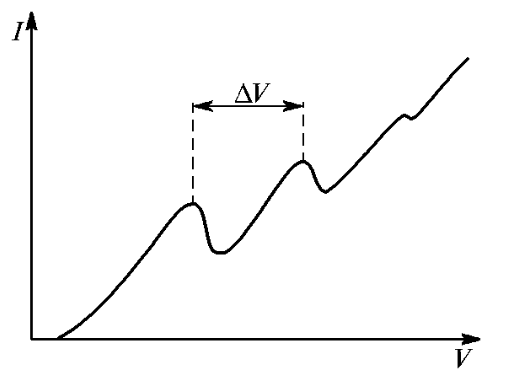
\includegraphics[width=1\textwidth]{gen/iv.pdf}
			\caption{График зависимости $\sqrt{U_I} (V)$ для 1 части спектра.}
		\end{minipage}
		\hfill
		\begin{minipage}[c]{0.48\textwidth}
			\centering
			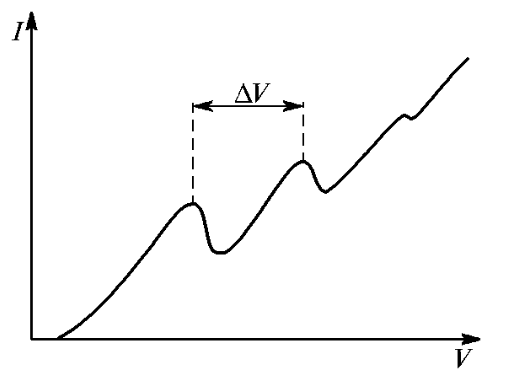
\includegraphics[width=1\textwidth]{gen/iv.pdf}
			\caption{График зависимости $\sqrt{U_I} (V)$ для 2 части спектра.}
		\end{minipage}
	\end{figure}

	Согласно теории $\sqrt{U_I} \propto V$. Методом наименьших квадратов построим аппроксимирующие кривые и определим величину задерживающего напряжения:
	
	\begin{table}[H]
		\centering
		\begin{tabular}{c}
			$\lambda = 7032.41 \angstrom, V_0 = (-0.28 \pm 0.01) В$ \\
			$\lambda = 6678.28 \angstrom, V_0 = (-0.33 \pm 0.02) В$ \\
			$\lambda = 6506.53 \angstrom, V_0 = (-0.37 \pm 0.02) В$ \\
			$\lambda = 6334.42 \angstrom, V_0 = (-0.42 \pm 0.02) В$ \\
			$\lambda = 6217.28 \angstrom, V_0 = (-0.45 \pm 0.02) В$ \\
			$\lambda = 6074.34 \angstrom, V_0 = (-0.54 \pm 0.03) В$ \\
			$\lambda = 5944.83 \angstrom, V_0 = (-0.54 \pm 0.03) В$ \\
			$\lambda = 5400.56 \angstrom, V_0 = (-0.79 \pm 0.04) В$	
		\end{tabular}
	\end{table}
	
	Построим график зависимости задерживающего напряжения от частоты излучения.			
	\begin{figure}[H]
		\centering
		\includegraphics[width=0.5\textwidth]{gen/v0_omega.png}
		\caption{График зависимости $U_0 (\omega)$.}
	\end{figure}

	С помощью метода наименьших квадратов проведём аппроксимирующую прямую. По коэффициенту наклона прямой $a$ определим постоянную Планка:
	$\hbar = a \cdot e = (1.03 \pm 0.06) \cdot 10^{-34} \; Дж \cdot с$
	
	Построим график зависимостей $U_I(V)$.
			
	\begin{figure}[H]
		\centering
		\includegraphics[width=0.5\textwidth]{gen/iv_full.png}
		\caption{График зависимости $U_I (V)$.}
	\end{figure}
	
	По графику видно, что с увеличением длины волны значение тока насыщения увеличивается, а величина задерживающего напряжения уменьшается.
	
	\subsection*{Обсуждение результатов и выводы}
	
	В работе была экспериментально подтверждена линейная зависимость корня из фототока от величины задерживающего напряжения:
	$$
	\sqrt{I} \propto V_{задерж}
	$$
	Была подтверждена линейная зависимость задерживающего напряжения от частоты падающего на фотоэлемент излучения:
	$$
	V_{задерж} \propto \omega
	$$
	Была определена постоянная Планка:
	$\hbar = (1.03 \pm 0.06) \cdot 10^{-34} \; Дж \cdot с$\\
	$\hbar_{теор} = 1.054...  \cdot 10^{-34}$
	В пределах погрешности теоретическое и измеренное значения совпадают.
	
	
\end{document}